\documentclass{article}
\usepackage{amsmath}
\usepackage{graphicx}
\usepackage{geometry}
\usepackage{amsfonts}
\usepackage{amssymb}
\usepackage{graphicx}
\usepackage[utf8]{inputenc} %Spanish input                                      
\usepackage[T1]{fontenc} % Use 8-bit encoding that has 256 glyphs 
\usepackage[spanish, es-tabla]{babel}        
\usepackage{float}
\usepackage{lscape}
\usepackage{enumerate}
\usepackage{color}
\usepackage{algpseudocode}
\usepackage{mathtools}
\usepackage{wrapfig}
\usepackage{subfig}
\usepackage{cite} % para contraer referencias
\usepackage{eurosym} % para el euro
\usepackage{setspace} % para el espacio de las filas de la tabla


%------------------------------------------------------------------------
\newtheorem{theorem}{Theorem}
\newtheorem{acknowledgement}[theorem]{Acknowledgement}
\newtheorem{algorithm}[theorem]{Algorithm}
\newtheorem{axiom}[theorem]{Axiom}
\newtheorem{case}[theorem]{Case}
\newtheorem{claim}[theorem]{Claim}
\newtheorem{conclusion}[theorem]{Conclusion}
\newtheorem{condition}[theorem]{Condition}
\newtheorem{conjecture}[theorem]{Conjecture}
\newtheorem{corollary}[theorem]{Corollary}
\newtheorem{criterion}[theorem]{Criterion}
\newtheorem{definition}[theorem]{Definition}
\newtheorem{example}[theorem]{Example}
\newtheorem{exercise}[theorem]{Exercise}
\newtheorem{lemma}[theorem]{Lemma}
\newtheorem{notation}[theorem]{Notation}
\newtheorem{problem}[theorem]{Problem}
\newtheorem{proposition}[theorem]{Proposition}
\newtheorem{remark}[theorem]{Remark}
\newtheorem{solution}[theorem]{Solution}
\newtheorem{summary}[theorem]{Summary}
\newenvironment{proof}[1][Proof]{\textbf{#1.} }{\ \rule{0.5em}{0.5em}}
\usepackage{fancyhdr}
\pagestyle{fancy}
\setlength{\textwidth}{7.0in}
\setlength{\oddsidemargin}{-0.35in}
\setlength{\topmargin}{-0.5in}
\setlength{\textheight}{9.0in}
\setlength{\parindent}{0.3in}
\setlength{\pdfpagewidth}{88.184mm}
\setlength{\pdfpageheight}{113.854mm}
\setlength{\footskip}{12.0pt}
\usepackage[hidelinks]{hyperref}
\usepackage{xstring}
\usepackage{listings}
\usepackage{lipsum}
\usepackage{courier}
\usepackage{multirow}
\usepackage{pdfpages}



\newcommand{\thelink}{\@empty}
\newcommand{\link}[2]{%
  \IfSubStr{#1}{:}{\renewcommand\thelink{#1}}{\renewcommand\thelink{#1:#2}}%
  \href{\thelink}{\texttt{#2}}%
}
%--------------------------------------------------------------
\geometry{
  a4paper,
  left=30mm,
  right=30mm,
  headheight=3cm,
  top=2.5cm,
  bottom=3.5cm,
  footskip=0cm
}
\begin{document}
\begin{titlepage}
\title{TSI PRACTICA 1}
\author{Pablo Huertas Arroyo}
\date{ \today }


\maketitle
\begin{figure}[h]
    \centering
    
\includegraphics[scale=4]{LogoUGR.png}
\end{figure}


\hspace{-1.7cm}
\newline Correo: \link{mailto}{phuertas@correo.ugr.es}
\newline DNI:77033078Y
\newline Grupo 3A, subgrupo 2
\newline Horario: Luneas de 17:30 a 19:30
\end{titlepage}

%\newpage
%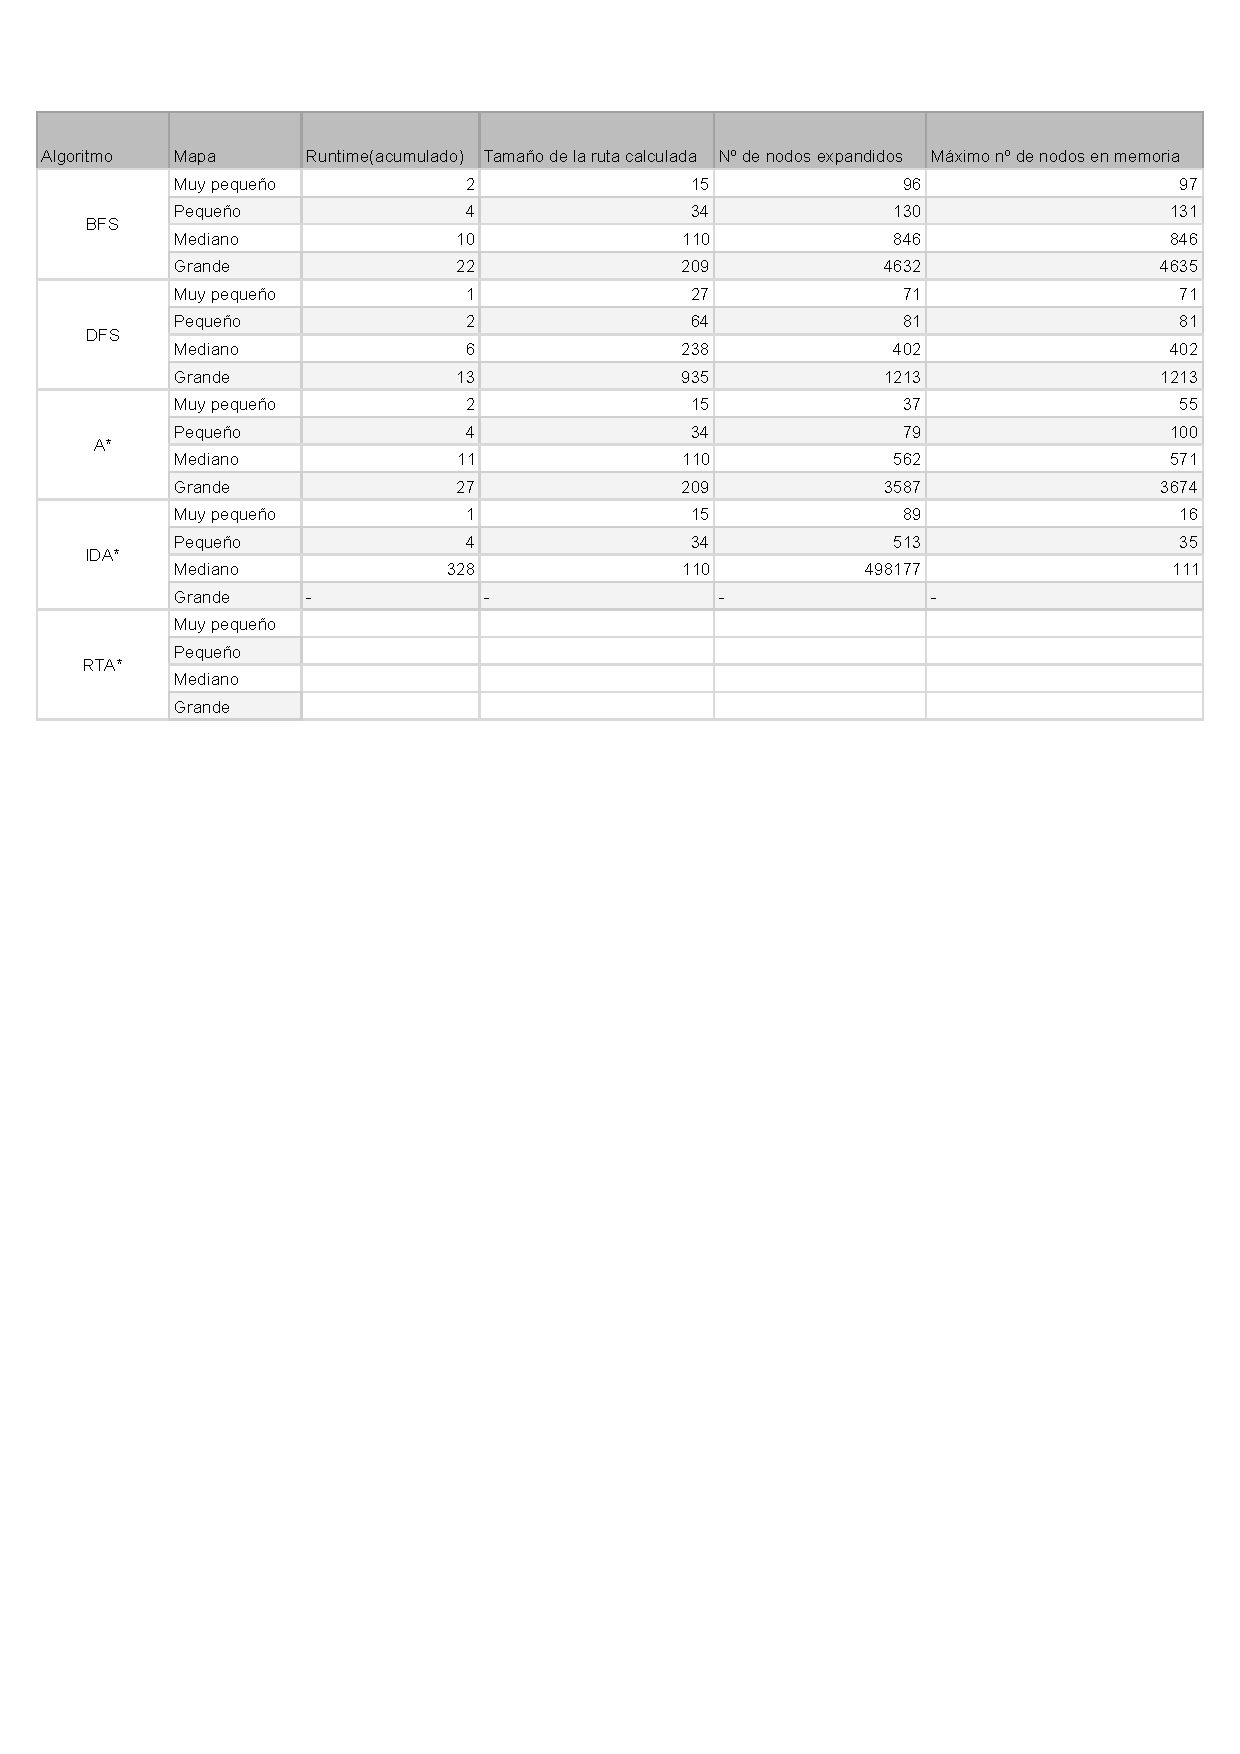
\includepdf[pages=-]{resultados.pdf}
%\vspace{10mm}

\newpage
\tableofcontents

%---------------------------------------------------------------------------------------------------------------------
%---------------------------------------------------------------------------------------------------------------------
% PROBLEMA DE LAS MONEDAS
%---------------------------------------------------------------------------------------------------------------------
%---------------------------------------------------------------------------------------------------------------------
\newpage
\section{\large{Problema de las monedas}}

\subsection{Apartado a}
\maketitle{\emph{\textbf{Se desea encontrar un conjunto de monedas cuyo importe sea exactamente una cantidad
dada. Para ello, se usarán las monedas de 1, 2, 5, 10, 20 y 50 céntimos, así como las de
1 y 2 euros. Codifique una solución en MZN que calcule cualquier solución válida, y
complete la siguiente tabla usando esta codificación:}}}

\vspace {1cm}

La tabla \ref{tab:tabmonedasA} muestra las soluciones conseguidas con la codificación (a) para el problema de las monedas.
\begin{table}[h]
  \begin{center}
    \begin{spacing}{1.5}
    \begin{tabular}{| p{1,5cm} | p{7cm} | p{4cm} | p{2cm} |}
      \hline
      Importe & {Primera solución encontrada y número de monedas en la misma} & Número total de soluciones & Runtime (en segundos) \\ \hline
      0,17 {\euro} & 
      \begin{tabular}{p{7cm}}
        cantidad = 17 \\
        monedas = 17; \\
        contador = [0, 0, 0, 0, 0, 0, 17]; \\
        centimos = [200, 100, 50, 20, 10, 5, 2, 1];
      \end{tabular}
      & 28 & 0'123 \\ \hline

      1,43 {\euro} & 
      \begin{tabular}{p{7cm}}
        cantidad = 143 \\
        monedas = 143 \\
        contador = [0, 0, 0, 0, 0, 0, 143] \\
        centimos = [200, 100, 50, 20, 10, 5, 2, 1]
      \end{tabular}
      & 17952 & 2'956\\ \hline

      2,35 {\euro} & 
      \begin{tabular}{p{7cm}}
        cantidad = 235 \\
        monedas = 235 \\
        contador = [0, 0, 0, 0, 0, 0, 0, 235] \\
        centimos = [200, 100, 50, 20, 10, 5, 2, 1]
      \end{tabular}
      & 150824 & 17'342\\ \hline

      4,99 {\euro} & 
      \begin{tabular}{p{7cm}}
        cantidad = 499 \\
        monedas = 499; \\
        contador = [0, 0, 0, 0, 0, 0, 499]; \\
        centimos = [200, 100, 50, 20, 10, 5, 2, 1];
      \end{tabular}
      & 6224452 & 258'87 \\ \hline
    \end{tabular}
    \end{spacing}
    \caption{Tabla de soluciones para el problema de las monedas(Apartado 1)}
    \label{tab:tabmonedasA}
  \end{center}
\end{table}

\newpage
\subsection{Apartado b}
\maketitle{\emph{\textbf{Modifique la versión anterior de forma que la parte entera de los importes sea asignada
únicamente a monedas de uno y dos euros. Por ejemplo, para el importe de 1,43€ se
deberá forzosamente asignar una moneda de 1€ y completar los 43 céntimos restantes
con monedas de 1, 2, 5, 10, 20 o 50 céntimos. Complete la tabla anterior con esta nueva
codificación}}}

\vspace {1cm}

La tabla \ref{tab:tabmonedasB} muestra las soluciones conseguidas con la codificación (b) para el problema de las monedas.
\begin{table}[h]
  \begin{center}
    \begin{spacing}{1.5}
    \begin{tabular}{| p{1,5cm} | p{7cm} | p{4cm} | p{2cm} |}
      \hline
      Importe & {Primera solución encontrada y número de monedas en la misma} & Número total de soluciones & Runtime (en segundos) \\ \hline
      0,17 {\euro} & 
      \begin{tabular}{p{7cm}}
        cantidad = 17 \\
        monedas = 17; \\
        contador = [0, 0, 0, 0, 0, 0, 17]; \\
        centimos = [200, 100, 50, 20, 10, 5, 2, 1];
      \end{tabular}
      & 28 & 0'166 \\ \hline

      1,43 {\euro} & 
      \begin{tabular}{p{7cm}}
        cantidad = 143 \\
        monedas = 44 \\
        contador = [0, 1, 0, 0, 0, 0, 43] \\
        centimos = [200, 100, 50, 20, 10, 5, 2, 1]
      \end{tabular}
      & 284 & 0'344\\ \hline

      2,35 {\euro} & 
      \begin{tabular}{p{7cm}}
        cantidad = 235 \\
        monedas = 36 \\
        contador = [1, 0, 0, 0, 0, 0, 0, 35] \\
        centimos = [200, 100, 50, 20, 10, 5, 2, 1]
      \end{tabular}
      & 162 & 0'229\\ \hline

      4,99 {\euro} & 
      \begin{tabular}{p{7cm}}
        cantidad = 499 \\
        monedas = 300; \\
        contador = [1, 0, 0, 0, 0, 0, 299]; \\
        centimos = [200, 100, 50, 20, 10, 5, 2, 1];
      \end{tabular}
      & 463212 & 68 \\ \hline
    \end{tabular}
    \end{spacing}
    \caption{Tabla de soluciones para el problema de las monedas(Apartado 2)}
    \label{tab:tabmonedasB}
  \end{center}
\end{table}

\newpage
\subsection{Apartado c}
\maketitle{\emph{\textbf{Realice una nueva modificación sobre la versión anterior para que el conjunto de
monedas encontrados sea mínimo, es decir, que tenga el menor número de monedas
posible. Para ello, se recomienda comenzar por la parte de satisfacción y guardar en una
variable la “cantidad” de monedas de la solución encontrada, y tras esto resolver la
parte de optimización usando la sentencia: solve minimize <variable>
\newline Genere una nueva tabla de resultados con una columna de “solución óptima” donde se
indique la solución óptima encontrada para los importes anteriores y la cantidad de
monedas de la misma, y otra columna de runtime.}}}

\vspace {1cm}

La tabla \ref{tab:tabmonedasC} muestra las soluciones conseguidas con la codificación (c) para el problema de las monedas.
\begin{table}[h]
  \begin{center}
    \begin{spacing}{1.5}
    \begin{tabular}{| p{1,5cm} | p{7cm} | p{4cm} | p{2cm} |}
      \hline
      Importe & {Solución óptima y número de monedas en la misma} & Número total de soluciones & Runtime (en segundos) \\ \hline
      0,17 {\euro} & 
      \begin{tabular}{p{7cm}}
        cantidad = 17 \\
        monedas = 3; \\
        contador = [0, 0, 0, 1, 1, 1, 0]; \\
        centimos = [200, 100, 50, 20, 10, 5, 2, 1];
      \end{tabular}
      & 15 & 0'156 \\ \hline

      1,43 {\euro} & 
      \begin{tabular}{p{7cm}}
        cantidad = 143 \\
        monedas = 5 \\
        contador = [0, 1, 0, 2, 0, 1, 1] \\
        centimos = [200, 100, 50, 20, 10, 5, 2, 1]
      \end{tabular}
      & 40 & 0'135\\ \hline

      2,35 {\euro} & 
      \begin{tabular}{p{7cm}}
        cantidad = 235 \\
        monedas = 4 \\
        contador = [1, 0, 0, 1, 1, 1, 0, 0] \\
        centimos = [200, 100, 50, 20, 10, 5, 2, 1]
      \end{tabular}
      & 32 & 0'138\\ \hline

      4,99 {\euro} & 
      \begin{tabular}{p{7cm}}
        cantidad = 499 \\
        monedas = 8; \\
        contador = [2, 0, 1, 2, 0, 1, 2, 0]; \\
        centimos = [200, 100, 50, 20, 10, 5, 2, 1];
      \end{tabular}
      & 293 & 0'117 \\ \hline
    \end{tabular}
    \end{spacing}
    \caption{Tabla de soluciones para el problema de las monedas(Apartado 3)}
    \label{tab:tabmonedasC}
  \end{center}
\end{table}


\newpage
\subsection{Cuestiones}
\maketitle{\emph{\textbf{Responda razonadamente a las siguientes cuestiones:}}}
\begin{description}
  \item[\begin{tabular}{p{15cm}}{¿Qué ocurriría si, usando la
  codificación (a) para encontrar todas las soluciones, el importe buscado es mucho
  mayor?}\end{tabular}]
    Seria computacionalmente imposible, ya que viendo lo que tarda con los 4'99 {\euro}, tenemos un 
    orden de complejidad excesivamente alto y creceria exponencialmente con el tamaño del problema.
    Deberíamos usar ciertas restricciones para encontrar restringir el espacio de búsqueda, y no 
    usar la fuerza bruta para encontrar todas las soluciones.

  \item [\begin{tabular}{p{15cm}}{¿Se podría encontrar alguna solución (usando la codificación de (a) o cualquier
  otra) de este problema con un importe del orden de los millones de euros?}\end{tabular}]
    Usando la codificación (a), tal y como hemos visto antes, tardaría un tiempo computacionalmente imposible de ser
    eficiente si queremos encontrar todas las soluciones y quedarnos con la mejor solución, pero si solo queremos encontrar
    una solución independientemente de la cantidad de monedas usadas, con la codificación de (a) podemos encontrar una solución
    de manera casi instantánea. Eso sí, la solución encontrada sería tanto números de monedas de 1 céntimo como sea el importe.

    En la codificación (b) también encuentra una solución de manera casi instantánea, debido a que la única restricción 
    que se tiene esque si el importe es mayor de 200 se use una moneda de 2 euros, y si es entre 100 y 200 se use una moneda de 1 euro.
    Por lo tanto, la restricción solo nos dice que tiene que haber una moneda de 2 euros con un caso de importe del millón de euros, pero tras 
    cumplirse esta restricción, se realiza una búsqueda de soluciones con fuerza bruta como en la codificación (a).

    En la codificación (c) sí encuentra una solución, pero tarda mucho más que las otras 2 (aproximadamente 7 minutos), ya que al usar el \emph{solve minimize monedas}, se va a encargar
    de encontrar la solución con menor número de monedas. Eso sí, si paramos la ejecución antes de que encuentre la mejor solución, si detenemos la ejecución,
    nos mostrará el resultado de la mejor solución encontrada por el momento.

  \item[\begin{tabular}{p{15cm}}{En caso afirmativo, ¿cuál podría ser una estrategia prometedora?}\end{tabular}]
    La mejor estrategia sería la codificación (c), ya que al final lo que queremos es encontrar la solución con menor número de monedas.
    Aún siendo la mejor codificación de las 3, añadiría ciertas condiciones para restringir mucho más el espacio de búsqueda, 
    como por ejemplo, en vez de decir que si el importe es mayor que 200, se use una moneda de 2 euros, tener una variable que sea el 
    cociente entre el importe y 200, y que se usen tantas monedas de 2 euros como sea la parte entera de dicho cociente.
    \emph{float: cant2euros = cantidad/200;
    constraint if cant2euros>=1 then contador[1]>=cant2euros}
    Por ejemplo, si hay un importe de 700, se usarán 700/200 = 3 monedas de 2 euros.
    De esta forma, la búsqueda de soluciones sería mucho más eficiente.

\end{description}



%---------------------------------------------------------------------------------------------------------------------
%---------------------------------------------------------------------------------------------------------------------
% PROBLEMA DE LOS HORARIOS
%---------------------------------------------------------------------------------------------------------------------
%---------------------------------------------------------------------------------------------------------------------
\newpage
\section {\large{Problema de los horarios}}
\maketitle{\emph{\textbf{Responda a las siguientes preguntas de forma razonada:}}}
\begin{description}
  \item[\begin{tabular}{p{15cm}}{¿Cuál es el número de soluciones
    válidas obtenidas?}\end{tabular}]
    El número de soluciones que he obtenido son 2, que se diferencian únicamente en el viernes las dos 
    últimas horas, donde alternan entre sí las asignaturas 2 y 7

    La soluciones obtenidas son:
    \begin{table}[h]
      \begin{center}
        \begin{spacing}{1.5}
        \begin{tabular}{| l | l | l | l | l | l | l |}
          \hline
          Lunes & 4 & 4 & 9 & 0 & 1 & 1\\ \hline
          Martes & 4 & 4 & 7 & 0 & 1 & 1\\ \hline
          Miércoles & 8 & 8 & 6 & 0 & 3 & 3\\ \hline
          Jueves & 5 & 5 & 2 & 0 & 3 & 3\\ \hline
          Viernes & 5 & 5 & 6 & 0 & 7 & 2 \\ \hline
        \end{tabular}
        \end{spacing}
        \caption{Primera solución obtenida}
      \end{center}
    \end{table}

    \begin{table}[h]
      \begin{center}
        \begin{spacing}{1.5}
        \begin{tabular}{| l | l | l | l | l | l | l |}
          \hline
          Lunes & 4 & 4 & 9 & 0 & 1 & 1\\ \hline
          Martes & 4 & 4 & 7 & 0 & 1 & 1\\ \hline
          Miércoles & 8 & 8 & 6 & 0 & 3 & 3\\ \hline
          Jueves & 5 & 5 & 2 & 0 & 3 & 3\\ \hline
          Viernes & 5 & 5 & 6 & 0 & 2 & 7 \\ \hline
        \end{tabular}
        \end{spacing}
        \caption{Segunda solución obtenida}
      \end{center}
    \end{table}

  \item [\begin{tabular}{p{15cm}}{¿Existen soluciones simétricas? Por soluciones simétricas se entienden
    aquellas que tienen valores distintos para las variables de la codificación CSP (por lo que
    MiniZinc las interpreta como soluciones diferentes), pero semánticamente representan la
    misma solución.}\end{tabular}]
    En mi caso no existen soluciones simétricas, ya que cada día de la semana tiene un vector independiente, por 
    lo que cada solución es una solución única. Por eso me salen las dos soluciones distintas.

  \item[\begin{tabular}{p{15cm}}{En caso de que la codificación propuesta contenga soluciones simétricas,
    ¿cómo se podrían evitar y cuál es el número de soluciones (no simétricas) obtenido? Explique
    cómo se consigue la rotura de simetrías (variables y/o restricciones utilizadas para ello), y
    entregue la solución MZN sin simetrías.}\end{tabular}]
    Como he comentado anteriormente, en mi caso no se obtienen soluciones simétricas, por lo que no se
    puede evitar.
    Respecto a cómo se consigue la rotura de simetría, existe varias formas de conseguir esto.
    \begin{itemize}
      \item Como he aplicado en este problema, que cada variable es la que es, es decir, que el primer día 
      es el lunes y el segundo es el martes, siempre, por lo que no se pueden intercambiar los días entre sí.
      Además. el array \emph{horas necesarias} identifica el número de horas obligatorias a la semana 
      inequivocamente, por lo que tampoco se pueden intercambiar entre sí.
      \item Añadir una restricción que obligue a que cada solución obtenida sea mejor 
      que la anterior
      \item Limitar el espacio de búsqueda, por ejemplo, usar variables discretas, o usar
      límites de valores para las variables, para que los árboles de búsqueda no sean
      tan extensos.
      \item El uso de restricciones redundantes, no añaden más información al modelo, pero si hacen que se limite
      el espacio de búsqueda.
    \end{itemize}

\end{description}
%---------------------------------------------------------------------------------------------------------------------
%---------------------------------------------------------------------------------------------------------------------
% PROBLEMA LOGICO
%---------------------------------------------------------------------------------------------------------------------
%---------------------------------------------------------------------------------------------------------------------
\newpage 
\section {\large{Problema lógico}}
\maketitle{\emph{\textbf{\begin{tabular}{p{15cm}}{Cinco personas de cinco regiones diferentes viven en las primeras cinco
casas contiguas de una calle. Practican cinco profesiones distintas, y cada uno tiene un animal y
una bebida favoritos, todos ello diferentes. Las casas están pintadas con diferentes colores.
Ademas sabemos lo siguiente:
\newline a. El vasco vive en la casa roja.
\newline b. El catalán tiene un perro.
\newline c. El gallego es un pintor.
\newline d. El navarro bebe te.
\newline e. El andaluz vive en la primera casa de la izquierda.
\newline f. El de la casa verde bebe café.
\newline g. La casa verde está al lado de la blanca y a su derecha.
\newline h. El escultor cría caracoles.
\newline i. El diplomático vive en la casa amarilla.
\newline j. En la casa central se bebe leche.
\newline k. La casa del andaluz está al lado de la azul.
\newline l. El violinista bebe zumo.
\newline m. El zorro está en una casa al lado de la del médico.
\newline n. El caballo está en una casa al lado de la del diplomático.
\newline Resolver el problema de forma que podamos responder: ¿dónde está la cebra y quién bebe
agua?}\end{tabular}}}}

\vspace {1cm}
\begin{tabular}{p{15cm}}{ La primera solución encontrada, es:
  \begin{itemize}
    \item La persona 1 es el escultor, que es vasco, que vive en la tercera casa, de color rojo, cuyo animal son los caracoles y su bebida favorita es leche.
    \item La persona 2 es el pintor, que es gallego, que vive en la quinta casa, de color verde, cuyo animal es la cebra y su bebida favorita es el café.
    \item La persona 3 es el diplomático, que es andaluz, que vive en la primera casa, de color amarillo, cuyo animal es el zorro y su bebida favorita es el agua.
    \item La persona 4 es el médico, que es navarro, que vive en la segunda casa, de color azul, cuyo animal es el caballo y su bebida favorita es el té.
    \item La persona 5 es el violinista, que es catalán, que vive en la cuarta casa, de color blanco, cuyo animal es el perro y su bebida favorita es el zumo.
  \end{itemize}
}\end{tabular}

\textbf{El número de soluciones encontradas son 120}

%---------------------------------------------------------------------------------------------------------------------
%---------------------------------------------------------------------------------------------------------------------
% PROBLEMA DE ASIGNACION DE TAREAS
%---------------------------------------------------------------------------------------------------------------------
%---------------------------------------------------------------------------------------------------------------------
\newpage 
\section {\large{Problema de asignación de tareas}}
No he conseguido al 100\% este ejercicio, solo conseguí la solución al tener solo un 
trabajador.

%---------------------------------------------------------------------------------------------------------------------
%---------------------------------------------------------------------------------------------------------------------
% PROBLEMA DE COLOREADO DE GRAFOS
%---------------------------------------------------------------------------------------------------------------------
%---------------------------------------------------------------------------------------------------------------------
\newpage 
\section {\large{Problema del coloreado de grafos}}

\maketitle{\emph{\textbf{El problema del coloreado de grafos consiste en
asignar un color a cada nodo del grafo de forma que dos nodos adyacentes no tengan el mismo
color, usando el mínimo número de colores. En este ejercicio se pide implementar una variante
de este problema: se debe asignar un color a cada arista de forma que dos aristas que compartan
algún nodo como extremo, deben tener colores diferentes.}}}
\vspace {1cm}

La tabla \ref{tab:tabcolores} muestra las soluciones conseguidas de media para cada caso del problema.
\begin{table}[ht]
  \begin{center}
    \begin{spacing}{1.5}
    \begin{tabular}{| l | l | l | }
      \hline
      Tamaño del grafo & {Número de colores mínimo} & Runtime (en segundos) \\ \hline
      N=4, M=6 & 3,2,3 $\rightarrow${2,66}  & 0'140  \\ \hline

      N=6, M=15 & 5,4,5 $\rightarrow${4,66} & 0'130 \\ \hline

      N=8, M=28 & 6,7,6 $\rightarrow${6,33} & 0'125 \\ \hline

      N=10, M=45 & 8,8,8 $\rightarrow${8} & 0'160 \\ \hline

      N=12, M=66 & 8,9,9 $\rightarrow${8,66} & 0'134 \\ \hline

      N=14, M=91 & 11,12,10 $\rightarrow${11} & 0'163 \\ \hline
    \end{tabular}
    \end{spacing}
    \caption{Tabla de soluciones para el problema de coloración de grafos}
    \label{tab:tabcolores}
  \end{center}
\end{table}

\begin{description}
  \item[\begin{tabular}{p{15cm}}{En base a los resultados obtenidos, ¿diría que este problema es escalable, es decir, se puede abordar su
    resolución en grafos de un tamaño considerable? Razone su respuesta.}\end{tabular}]
    Realizando pruebas, a partir de un número de nodos aproximadamente de 100, empiezan a empeorar los tiempos de forma bastante rápida.
    Por ejemplo con N=100, M=1000, se obtiene un tiempo de resolución de casi unos 4 segundos, y si aumentamos el número de nodos a 120 sube hasta 
    unos 10 segundos, disparándose a 1 minuto si llegamos a  los 150 nodos.
    Podemos ver una curva exponencial a partir de estos datos por lo que podemos afirmar que no es un problema escalable, ya que 
    en un cierto punto de la curva el tiempo de resolución aumenta exponencialmente por lo que con tamaños de problema realmente grandes 
    sería computacionalmente imposible resolverlo.
\end{description}

\end{document}